\subsection{Introduction}
Dans ce premier TP nous allons mettre en évidence qu'avec une protection trop simple 
il est relativement simple d'obtenir des informations lors d'un chiffrement de données 
sensibles.\\

Durant ce TP, le code source d'une IP d'un AES nous est fourni. 
Celle-ci permet de chiffrer ou déchiffrer un message à partir d'une clé secrète. 
Nous allons donc simuler l'injection d'une faute par un laser sur le {\em "chemin"} 
emprunté par les données lors des multiples rondes de l'AES. Pour rester 
réaliste, nous ferons un {\em bit-flip} 8 bits (1 octet) une et une seule fois.

\subsection{Quelles protections sont mises en place contre les attaques par fautes?}

Bien que l'algorithme de l'AES soit incassable aujourd'hui, son implémentation
peut permettre de récupérer des données sensibles par de nombreux moyens.
Dans ce TP, on s'intéresse à une potentielle attaque par injection de fautes et
à une contre-mesure de cette attaque.
Pour mener une attaque par faute dans ce module AES, nous avons tout d'abord
analysé le circuit et tenté de comprendre comment le système était protégé.\\

La sécurité du chiffrement tel qu'il est implémenté pour ce TP réside dans la
redondance d'information.
En effet, chaque calcul sur les octets du data\_unit est fait 2 fois, cela
permet, à l'issue des deux calculs, de comparer que les 2 résultats sont
identiques.
Dans ce cas, aucune faute ne sera détectée. En revanche, si l'un des deux
calculs ne donne pas le même résultat, un flag sera levé, et le calcul sera
considéré comme erroné.\\

De plus, il est possible de doubler le nombre de calculs effectués par ronde,
sans pour autant doubler le temps de calcul.
En effet, la figure~\ref{fig:DDR} page~\pageref{fig:DDR} montre que
durant les 6 premiers cycles, 12 calculs sont effectués (sur fronts montants et
descendants) et sur les 6 cycles suivants, 
les mêmes calculs sont à nouveau effectués.
Ainsi si l'assaillant change un octet du circuit, le calcul effectué sur les 6
premiers cycles et celui effectué sur les 6 derniers seront surement différents et
une erreur sera levée.

\begin{figure}[!htbp]
	\begin{center}
		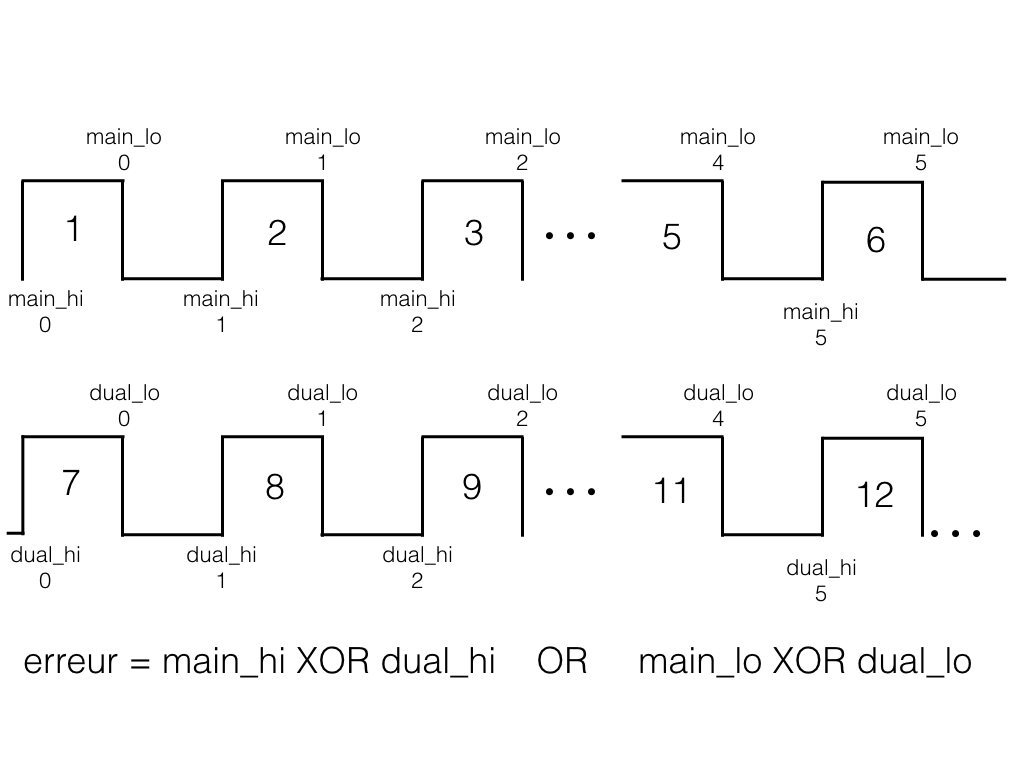
\includegraphics[scale=0.3]{AES/DDR}
		\caption{Exemple de Double Data Rate}
		\label{fig:DDR}
	\end{center}
\end{figure}

\subsection{Quelles sont les faiblesses de cette sécurité?}

Le problème avec cette façon de sécuriser l'AES est que si l'on change la valeur
d'un octet pendant exactement 6 cycles, la valeur du premier calcul sera
identique au deuxième calcul.
Ainsi, il ne sera plus possible de faire remonter l'erreur. 
Pour cela, l'attaquant doit parvenir à changer un octet durant l'un des tours de 
l'AES de telle sorte que main\_hi = dual\_hi et main\_lo = dual\_lo.
Si l'injection de la faute dure 6 cycles (temps nécessaire pour calculer
main\_hi et dual\_hi ainsi que main\_lo et dual\_lo) alors on peut être sûr que 
l'attaque sera réussie.

\subsection{Implémentation de l'attaque par faute}

Pour mettre en place notre attaque et tenter de la décrire nous avons réalisé 
un schéma (cf. figure~\ref{fig:AES} page~\pageref{fig:AES}).

\begin{figure}[!h]
	\begin{center}
		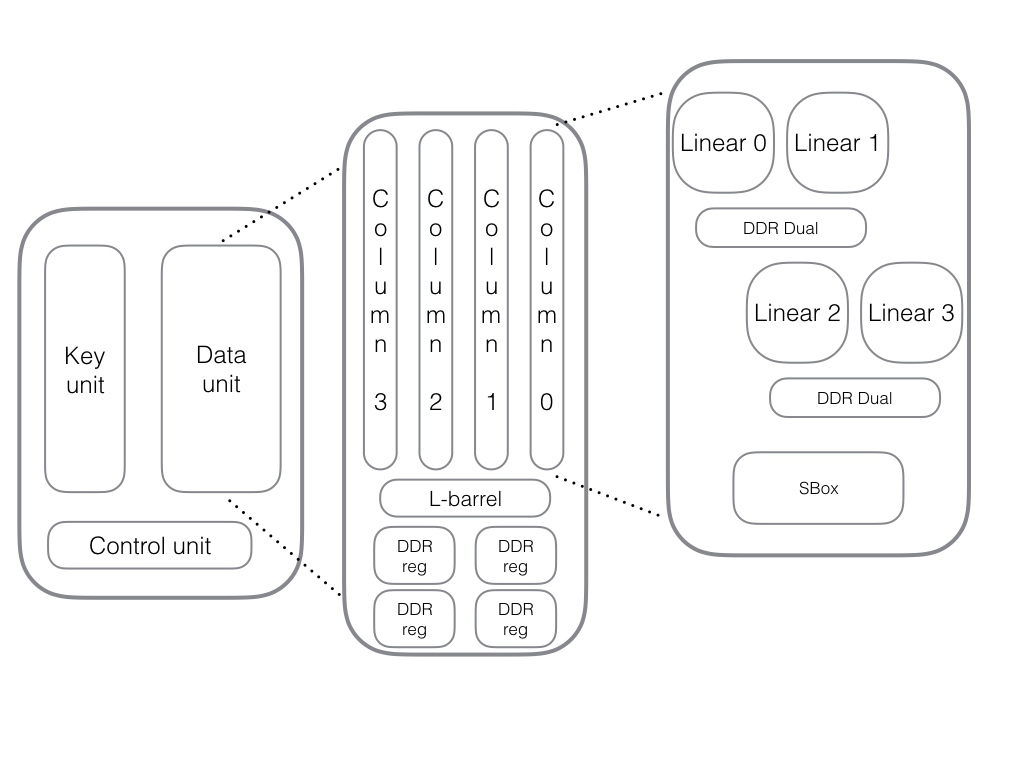
\includegraphics[scale=0.2]{AES/AES}
		\caption{Schéma simplifié de l'AES en différents niveaux d'abstractions}
		\label{fig:AES}
	\end{center}
\end{figure}

En utilisant la faiblesse expliquée précédemment, notre implémentation
consiste à introduire une faute de retournement de 8 bits sur le signal
\texttt{in\_hi\_sig} de la colonne 0, juste avant le bloc \texttt{linear}
(cf. figure~\ref{fig:AES} page~\pageref{fig:AES}).\\
Pour trouver le signal qui sera notre cible d'attaque nous avons 
simulé l'IP et modifié certains bits durant un chiffrement de l'AES. 
D'après la figure~\ref{fig:freeze} page~\pageref{fig:freeze} seul le changement 
de bits sur in\_hi n'a pas levé d'erreurs. En effet, dans ce cas, le main\_hi et le dual\_hi 
sont strictement identiques, ainsi le check\_dual est à 1 et aucune erreur n'est levée. 
Au contraire, lorsque l'on modifie un bit du main\_hi, le dual\_hi est différent 
et une erreur sera levée.\\

\begin{figure}[!h]
	\begin{center}
		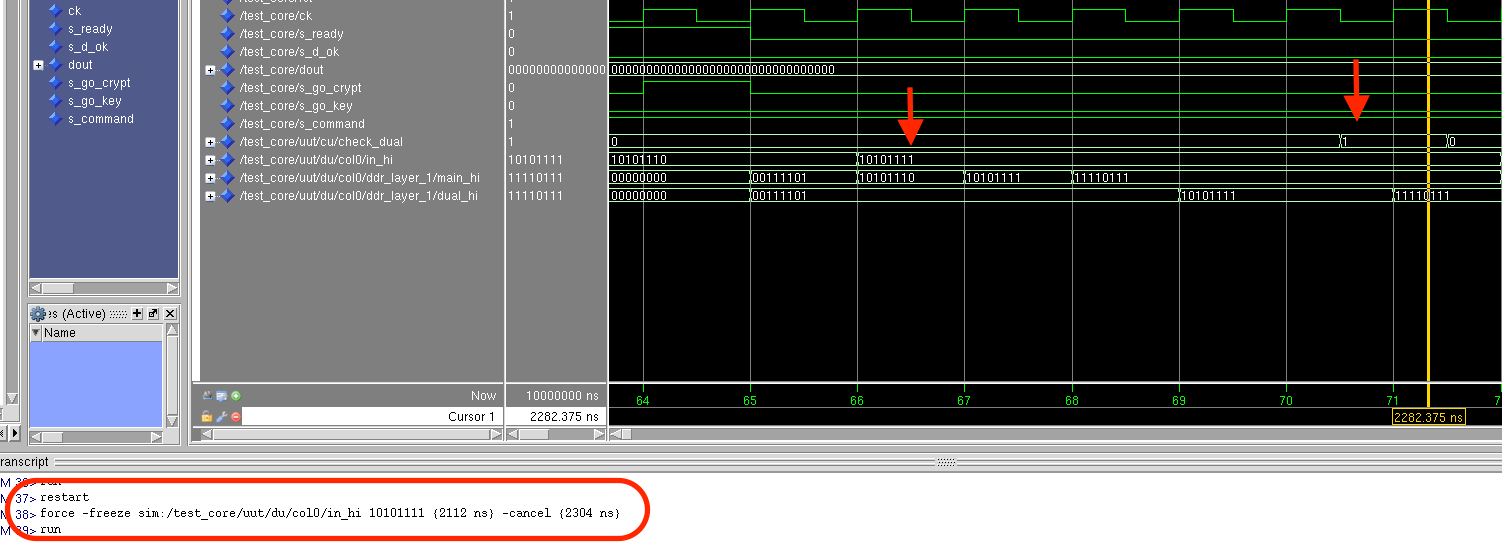
\includegraphics[scale=0.3]{freeze_in_hi}
		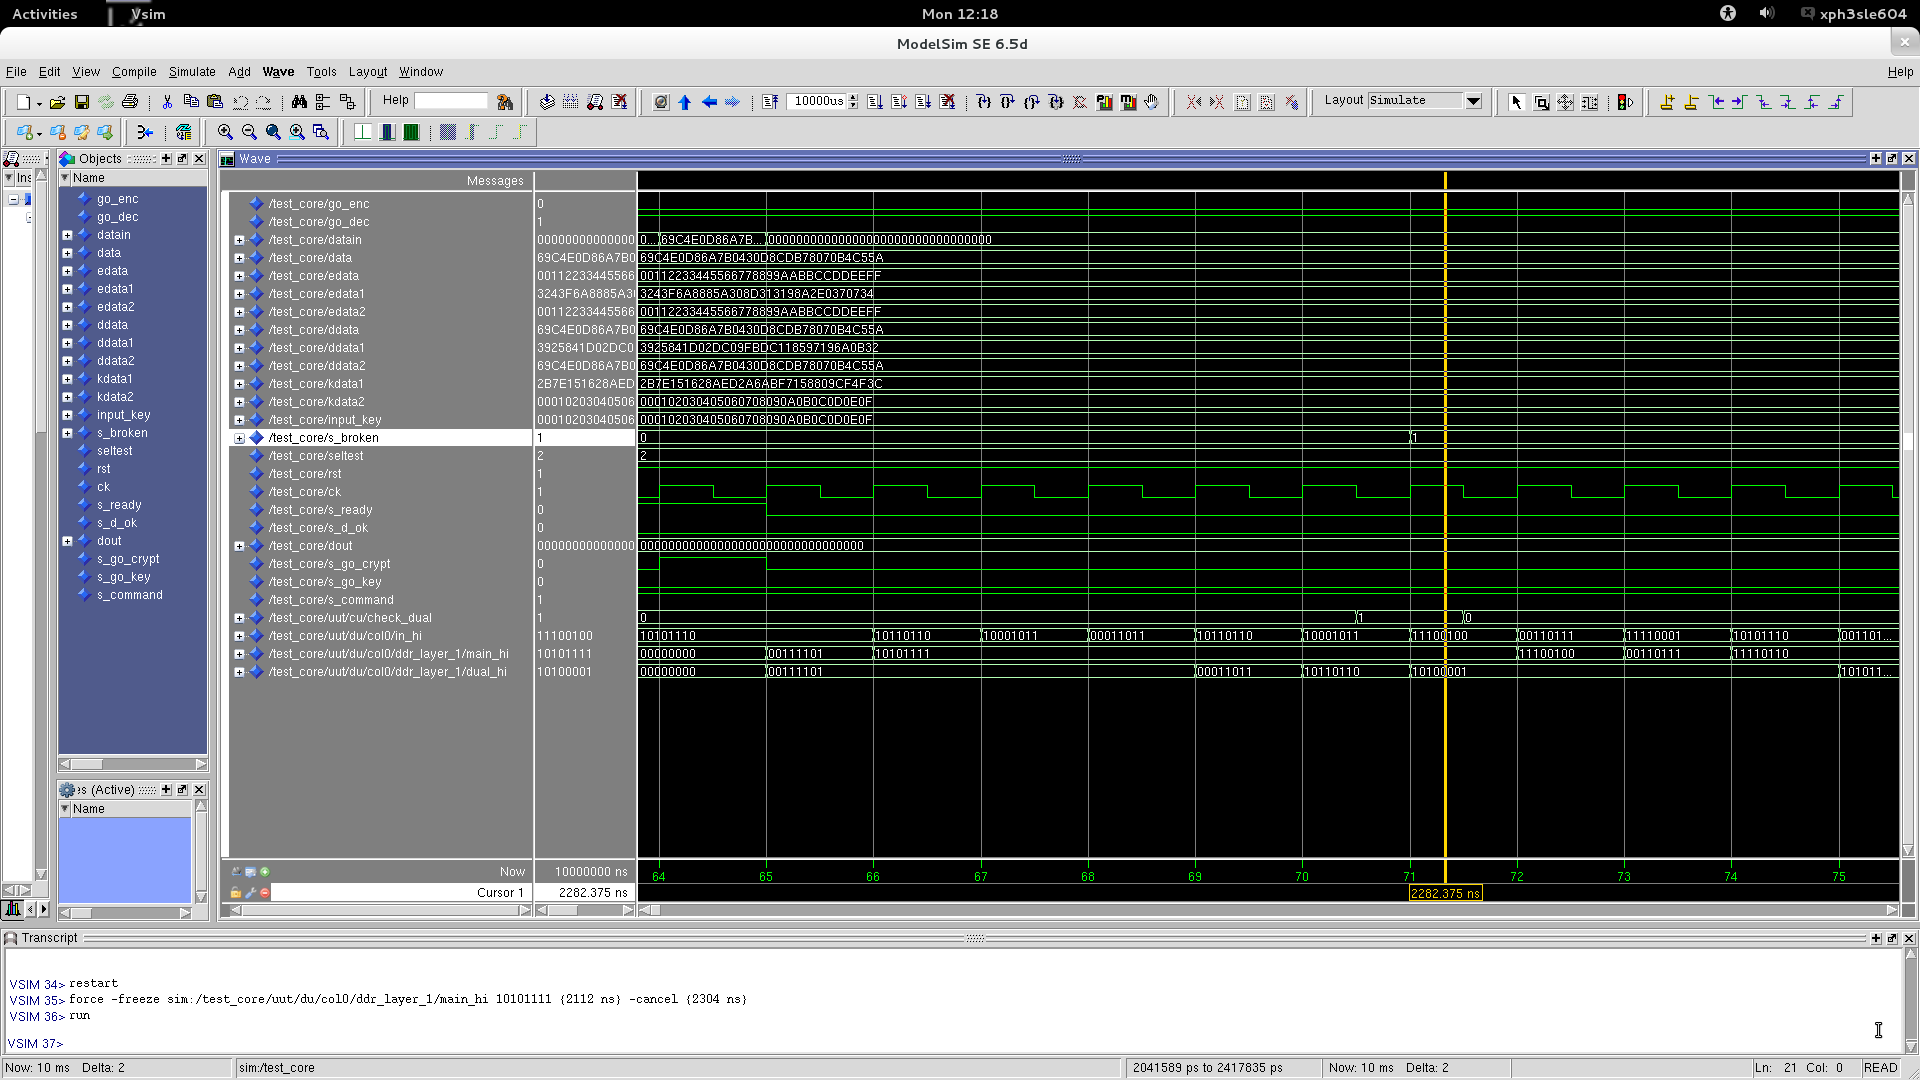
\includegraphics[scale=0.3]{freeze_main_hi}
		\caption{Simulation de bit-flip sur main\_hi et in\_hi. 
		Seule l'attaque de in\_hi durant 6 cycles ne lève pas d'erreurs.}
		\label{fig:freeze}
	\end{center}
\end{figure}

Nous nous basons sur un modèle réaliste d'injection de faute où, 
grâce à un laser, l'attaquant pourrait retourner les 8 bits de ce signal.\\
\texttt{in\_hi\_sig <= in\_hi;\\  lin\_0\_in <= in\_hi\_sig XOR fault\_sig;} \\
Le signal \texttt{fault\_sig} est remonté jusque dans le fichier top, comme un
port du composant \texttt{aes\_core}, pour pouvoir générer l'attaque.
Grâce au XOR, un bit à 1 dans le signal \texttt{fault\_sig} retournera le bit 
correspondant dans le signal \texttt{in\_hi} et injectera une faute.
Précisons que nous n'attaquons que la première colonne du DataUnit et que ce
même signal \texttt{fault\_sig} est laissé à \texttt{"00000000"} pour les trois
autres colonnes. \\
Nous avons tout d'abord testé cette implémentation en modifiant le test bench
VHDL qui instancie notre IP. Nous avons rajouté un process \texttt{fault},
qui incrément un compteur à chaque front montant et qui le remet à zéro à
chaque début de chiffrement. Après un certain nombre de cycles (peu important), nous injectons
la faute de retournement de bit (signal \texttt{fault\_sig} à
\texttt{"11111111"}), pendant exactement 6 cycles afin que les deux 
registres DDR (main et dual) soient affectés par l'attaque. \\
En utilisant les données fournies par la publication 197 du FIPS (Federal
Information Processing Standard), c'est à dire le texte d'entrée, 
la clé et le texte chiffré, nous pouvons vérifier que notre implémentation fonctionne. 
Si c'est la cas, la donnée d'entrée ne doit jamais changer pendant le chiffrement, le signal
de sortie de \texttt{aes\_core}, \texttt{error}, ne doit jamais passer à 1 et
la donnée de sortie doit être différente de la donnée attendue. \\
Nous avons obtenu de tels résultats (voir figures~\ref{modified_start} page~\pageref{modified_start} et
\ref{modified} page~\pageref{modified}) la donnée chiffrée, n'est pas celle attendue, le signal
\texttt{s\_broken} reste toujours à 0 et la donnée en entrée ne change pas. On
peut aussi voir que le signal modélisant le retournement de bit, \texttt{fault\_sig},
n'est actif que sur 6 cycles.

\begin{figure}[!h]
	\begin{center}
	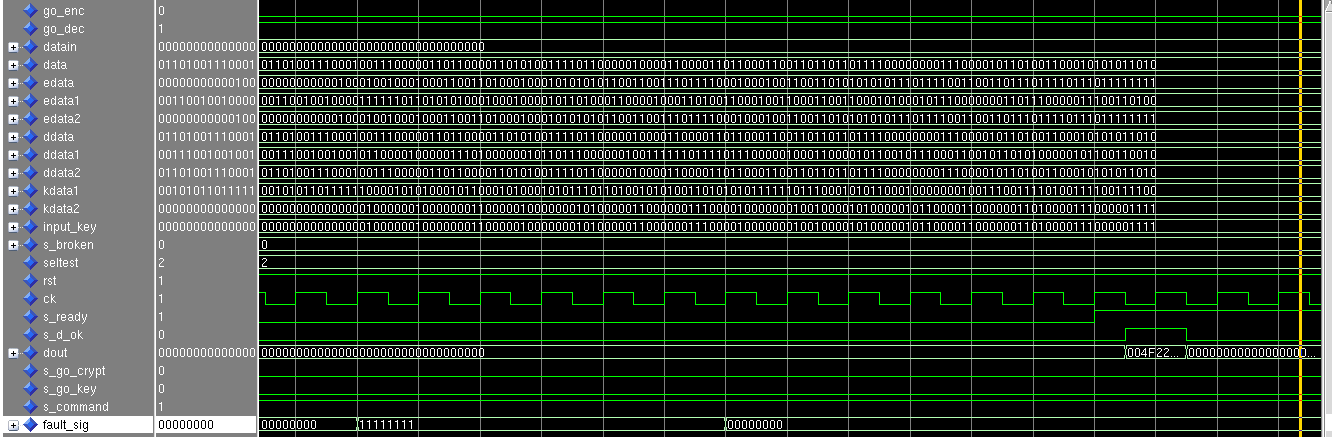
\includegraphics[scale=0.4]{result_modified_no_broken.png}
	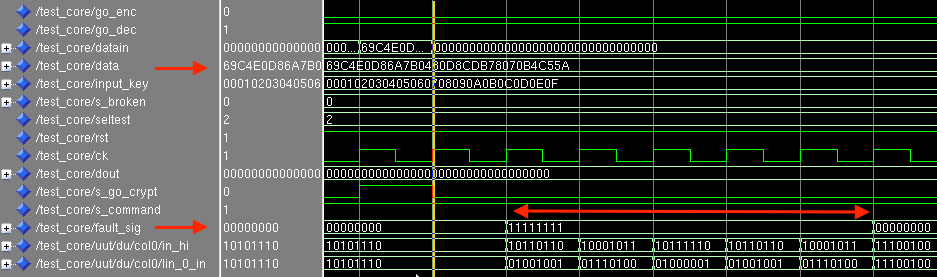
\includegraphics[scale=0.4]{result_modified_no_broken_start.png}
	\caption{Simulation de l'attaque par faute}
	\label{modified_start}
	\label{modified}
	\end{center}
\end{figure}

\begin{minipage}{\textwidth}
\subsection{Embarcation du code}

Nous avons embarqué notre IP dans un design développé par l'outil Xilinx EDK
et du code embarqué sur un processeur MicroBlaze. Nous avons tout d'abord testé
le comportement normal sans faute. Un petit morceau logiciel permet de configurer
l'IP grâce à différents registres : la clé, le texte et le mode
choisi (chiffrement/déchiffrement). L'IP repère les fronts montants sur certains
bits de registres pour charger la clé/lancer le processus. La figure \ref{post}
nous montre ce fonctionnement normal avec les mêmes données du FIPS pour un chiffrement.

Pour simuler l'erreur, on utilise le même process VHDL que dans le test bench
mais dans le fichier \texttt{user\_logic.vhd}. Ce process est aussi déclenché
avec un front montant sur un bit d'un registre. 

\begin{lstlisting}[language=VHDL]
-- for injection
   FAULT_INJECT : process( aes_clk ) is
-- init a 10 pour injecter qu'apres le 1er go crypt
   variable cycle_count : natural := 7 + ROUND_NUMBER * 6;
   begin 
      if aes_clk'event and aes_clk = '1' then
         if ( slv_reg0(3)='1' ) then
            cycle_count := cycle_count + 1;
            if s_go_crypt = '1' then
               cycle_count := 0;
            end if;
            if cycle_count > 1 + ROUND_NUMBER * 6 
            	and cycle_count < 7 + ROUND_NUMBER * 6 then
               fault_sig <= "11111111";
            else 
               fault_sig <= "00000000";
            end if;
         end if;
   end if;
\end{lstlisting}

\end{minipage}

\begin{figure}[h!]
	\begin{center}
	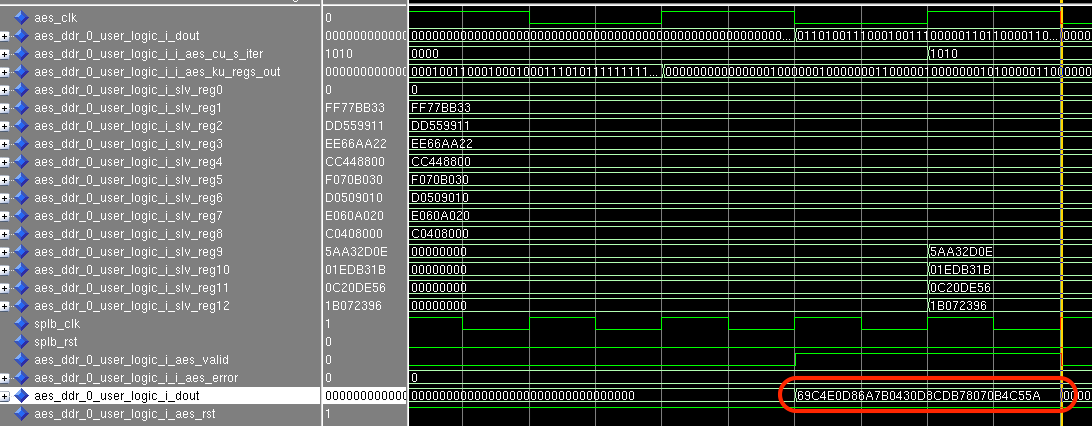
\includegraphics[scale=0.4]{post_synth.png}
	\caption{Simulation de l'IP embarquée pour un chiffrement de 
		00112233445566778899 et la clé 
		000102030405060708090A0B0C0D0E0F1012131415161718191A1B1C1D1E1F}
	\label{post}
	\end{center}
\end{figure}

Une fois le contrôle de l'attaque mis en place, il ne suffisait plus qu'à
lancer un synthèse pour que notre IP soit synthétisée. A l'issue, nous avons pu
faire un simulation post-synthèse en simulant le microblaze. Nous avons pu ainsi
observer, comme nous l'avions vu avant synthèse, que le résultat du chiffrement
est modifié par notre attaque, alors qu'aucun flag d'erreur n'est levé.

% Code en C pour contrôler l'IP à travers les registres, processeur MicroBlaze

\subsection{Conclusion}

Ce TP était une bonne occasion de découvrir de façon pratique une attaque
d'un système embarqué, l'attaque par injection de faute.
Il nous a aussi permis de mieux comprendre le fonctionnement interne de
l'algorithme AES.
